\begin{figure}[t]
\centering

\begin{subfigure}{0.48\linewidth}
\centering
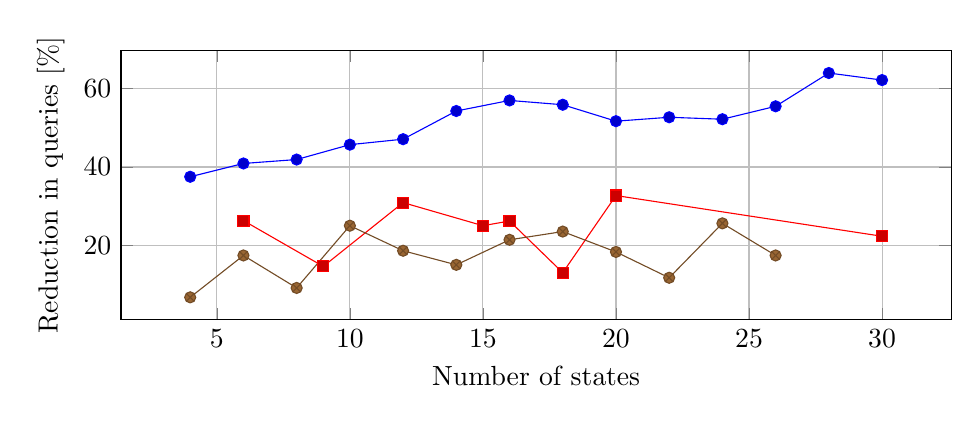
\begin{tikzpicture}
\begin{axis}[
    width=\linewidth,
    height=5cm,
    xlabel={Number of states},
    ylabel={Reduction in queries [\%]},
    legend to name=sharedlegend,
    legend columns=3,
    grid=both
]

% === Cancellation ===
\addplot coordinates {
    (4, 37.5)
    (6, 40.9)
    (8, 41.9)
    (10, 45.7)
    (12, 47.1)
    (14, 54.3)
    (16, 57.0)
    (18, 55.9)
    (20, 51.7)
    (22, 52.7)
    (24, 52.2)
    (26, 55.5)
    (28, 64.0)
    (30, 62.2)
};
\addlegendentry{Cancellation}

% === Commutativity ===
\addplot coordinates {
    (6, 26.3)
    (9, 14.6)
    (12, 30.9)
    (15, 25.0)
    (16, 26.2)
    (18, 13.0)
    (20, 32.7)
    (30, 22.3)
};
\addlegendentry{Commutativity}

% === Idempotency ===
\addplot coordinates {
    (4, 6.7)
    (6, 17.4)
    (8, 9.1)
    (10, 25.0)
    (12, 18.6)
    (14, 15.0)
    (16, 21.4)
    (18, 23.5)
    (20, 18.3)
    (22, 11.7)
    (24, 25.6)
    (26, 17.4)
};
\addlegendentry{Idempotency}

\end{axis}
\end{tikzpicture}
\caption{Reduction in the number of queries}
\end{subfigure}
\hfill
\begin{subfigure}{0.48\linewidth}
\centering
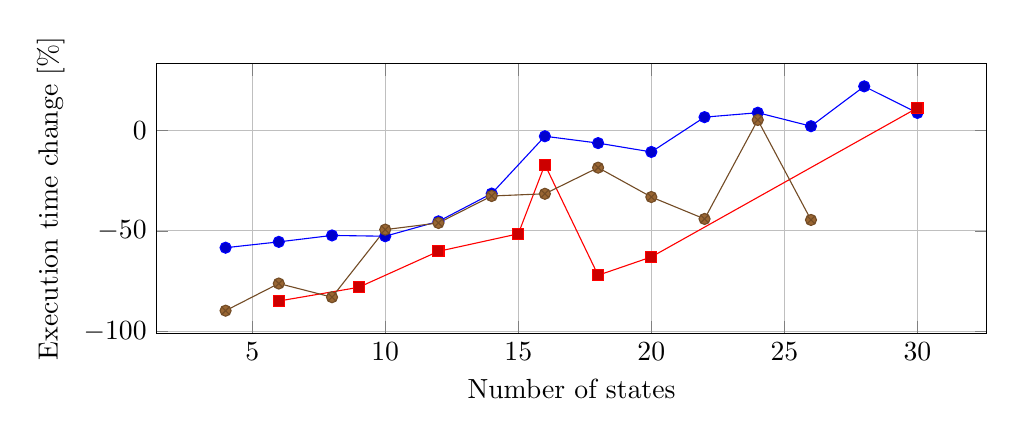
\begin{tikzpicture}
\begin{axis}[
    width=\linewidth,
    height=5cm,
    xlabel={Number of states},
    ylabel={Execution time change [\%]},
    grid=both
]

% === Cancellation ===
\addplot coordinates {
    (4, -58.4)
    (6, -55.5)
    (8, -52.3)
    (10, -52.7)
    (12, -45.3)
    (14, -31.5)
    (16, -3.0)
    (18, -6.4)
    (20, -10.8)
    (22, 6.5)
    (24, 8.7)
    (26, 2.0)
    (28, 21.8)
    (30, 8.6)
};

% === Commutativity ===
\addplot coordinates {
    (6, -84.9)
    (9, -78.1)
    (12, -60.2)
    (15, -51.5)
    (16, -17.1)
    (18, -72.1)
    (20, -63.0)
    (30, 11.1)
};

% === Idempotency ===
\addplot coordinates {
    (4, -89.7)
    (6, -76.2)
    (8, -83.0)
    (10, -49.4)
    (12, -46.1)
    (14, -32.7)
    (16, -31.6)
    (18, -18.6)
    (20, -33.2)
    (22, -44.1)
    (24, 5.1)
    (26, -44.6)
};

\end{axis}
\end{tikzpicture}
\caption{Relative change in execution time}
\end{subfigure}

\vspace{2mm}
\ref{sharedlegend}

\caption{Impact of SRS on the number of equivalence queries and execution time across different SRS rule types}

\end{figure}

\FloatBarrier